\documentclass{beamer}
%\documentclass[draft]{beamer}
%\documentclass[handout]{beamer}
\usepackage[latin1]{inputenc}
%\usepackage[ngerman]{babel}
\usepackage[english]{babel}

\usetheme{Boadilla}
\usefonttheme{professionalfonts}
\setbeamercovered{transparent}
\beamertemplatenavigationsymbolsempty
\setbeamertemplate{footline}[frame number]
\useinnertheme{rectangles}
\setbeamertemplate{blocks}[rounded][shadow=false]

\usepackage{enumerate} %% math
\usepackage{amsmath, amssymb} %%math
\usepackage{ulem} %%strike \sout{...}

\usepackage{tikz}
\usepackage{pgfpages}
\pgfpagesuselayout{resize to}[a4paper,border shrink=5mm,landscape]
\definecolor{orange}{RGB}{255,127,0}
\usepackage{listings}
\lstset{numbers=left,
	numberstyle=\footnotesize,
	numbersep=5pt,
	breaklines=true,
	showstringspaces=false,
	frame=l ,
	xleftmargin=15pt,
	xrightmargin=15pt,
	basicstyle=\ttfamily\small,
	stepnumber=1,
	keywordstyle=\color{blue},          % keyword style
  	commentstyle=\color{orange},       % comment style
%  	stringstyle=\color{green}         % string literal style
}
%Sprache Festelegen
\lstset{language=Python}
%\pgfpagesuselayout{two screens with lagging second} %% Pr�?sentation
%\pgfpagesuselayout{2 on 1}[a4paper,border shrink=5mm]
%\pgfpagesuselayout{4 on 1}[a4paper,border shrink=5mm, landscape]

%\pgfdeclareimage[width=.5\linewidth]{myimage}{images/myimage.png} % \pgfuseimage{myimage}

\pdfinfo{
  /Author (Robert M�ller, Christian Lemke, Max Wagner, Mattes Wieben)
  /Title (Normalverteilung)
  /Subject (Normalverteilung)
  /Keywords (Normalverteilung)
}

 
\title{Normalverteilung}
\subtitle{Master Practical Course ``Data Analysis with Python''\\(WiSe 2016/17)}
%\titlegraphic{\includegraphics[width=0.15\textwidth]{./raspberry_pi_python_logo.png}} 
\institute{
  Lehr- und Forschungseinheit f�r Programmier- und Modellierungssprachen\\
  Institut f�r Informatik\\
  Ludwig-Maximilians-Universit�t M�nchen\\[2em]
}

\author{Robert M�ller, Christian Lemke, Max Wagner, Mattes Wieben}
\date{06. Dezember 2016}

 
\begin{document}
%%%%%%%%%%%%%%%%%%%%%%%%%%%%%%%%%%%%%%%%%%%%%%%%%%%%%%%%%%%%%%%%%%%%%%%%%%%%%%%%
\begin{frame}
  \titlepage
\end{frame}


%%%%%%%%%%%%%%%%%%%%%%%%%%%%%%%%%%%%%%%%%%%%%%%%%%%%%%%%%%%%%%%%%%%%%%%%%%%%%%%%
\begin{frame}
  \frametitle{Agenda}
  \tableofcontents
\end{frame}


\section{Allgemeine Grundlagen}
%%%%%%%%%%%%%%%%%%%%%%%%%%%%%%%%%%%%%%%%%%%%%%%%%%%%%%%%%%%%%%%%%%%%%%%%%%%%%%%%
\begin{frame}
  \frametitle{Allgemeine Grundlagen}
  \begin{block}{}
    \begin{itemize}
      \item Beschreiben von Zufallsvariablen
      \item Bekannt als Gau�-Kurve
      \item Gepr�gt durch de Moivre, Laplace/Poisson und Gau�
      \item Approximiert Binomialverteilung
    \end{itemize}
  \end{block}
  \begin{figure}
    \centering
      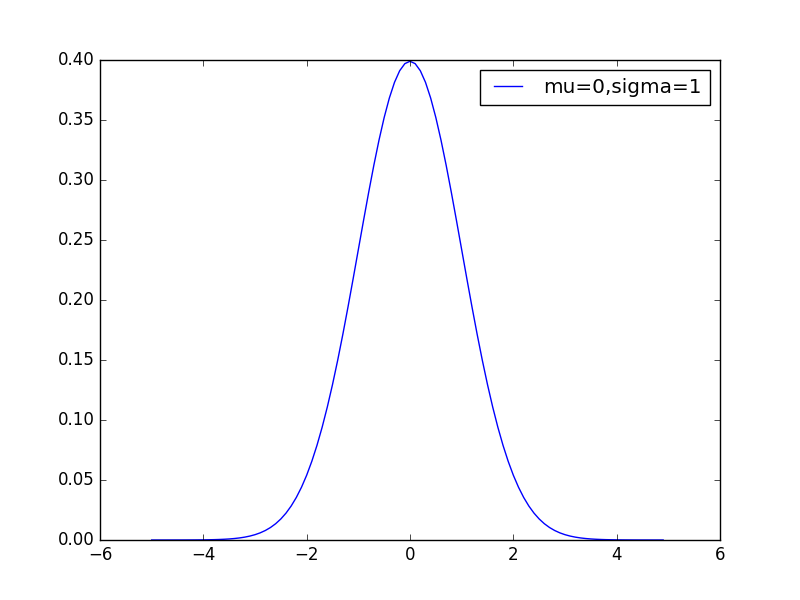
\includegraphics[width = 0.5\textwidth]{Standard.png}
  \end{figure}
\end{frame}

%%%%%%%%%%%%%%%%%%%%%%%%%%%%%%%%%%%%%%%%%%%%
\section{Mathematische Grundlagen}
\begin{frame}
  \frametitle{Mathematische Grundlagen}
  Sei \(X\) eine diskrete Zufallsvariable, wobei \(A\) die Menge der m�glichen Werte beschreibt, die \(X\) annehmen kann, dann gilt:
  \begin{block}{}
    \begin{itemize}
      \item Erwartungswert \(\mu(X) = \sum_{x \in A}(x*P(X=x))\) \\
      \item Varianz \(V(X) = \sum_{x\in A}((x-\mu)^2*P(X=x))\)
      \item Standardabweichung \(\sigma(X) = \sqrt{V(X)}\)
    \end{itemize}
  \end{block}
  Ein M�nzwurf w�re zum Beispiel eine diskrete Verteilung.
\end{frame}

\begin{frame}
  \frametitle{Beispiele}
  
    \begin{table}[h!]
    \centering
    \caption{M�nzwurf}
    \begin{tabular}{l||c|c}
      Ergebnis & Kopf & Zahl\\
      \hline
      Wahrscheinlichkeit & 1/2 & 1/2\\
    \end{tabular}
  \end{table}
  
    \begin{table}[h!]
    \centering
    \caption{W�rfel}
    \begin{tabular}{l||c|c|c|c|c|c}
      Ergebnis & 1 & 2 & 3 & 4 & 5 & 6\\
      \hline
      Wahrscheinlichkeit & 1/6 & 1/6 & 1/6 & 1/6 & 1/6 & 1/6\\
    \end{tabular}
  \end{table}
  
  \begin{block}{Stetige Wahrscheinlichkeitsverteilungen}
    F�r stetige Verteilungen w�re die Wahrscheinlichkeit jedoch immer nahe 0.\\
    \(\rightarrow\) Daher werden diese Verteilungen in einer Dichtefunktion angegeben
  \end{block}
\end{frame}

%%%%%%%%%%%%%%%%%%%%%%%%%%%%%%%%%%%%%%%%%%%%
\section{Dichtefunktion}
\begin{frame}
\frametitle{Dichtefunktion}
  \begin{block}{}
    \begin{equation}
      f(x\big\vert\mu,\sigma) = \frac{1}{\sqrt{2\pi\sigma^2}}e^{-\-\frac{(x-\mu)^2}{2\sigma^2}}
    \end{equation}
  \end{block}
  \begin{figure}
    \centering
      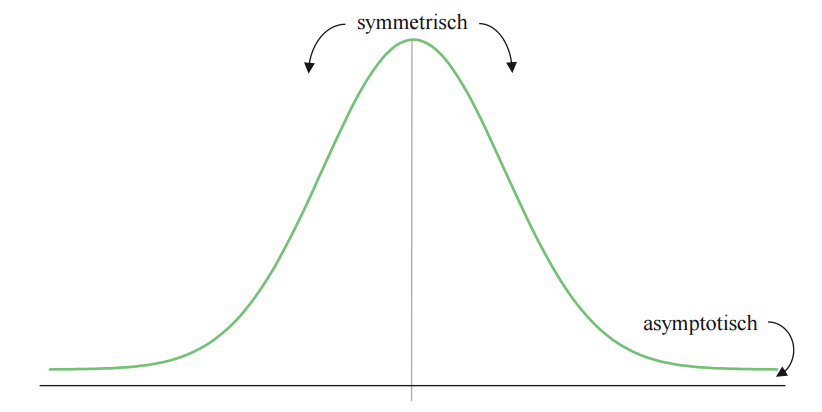
\includegraphics[width = 0.9\textwidth]{Eigenschaften.png}
    \caption{Gau�-Kurve\footnote{Franz Kronthaler: Statistik angewandt (2014) S. 110}}
    \label{2}
  \end{figure}
\end{frame}

\begin{frame}
\frametitle{Dichtefunktion}
  \begin{block}{Wahrscheinlichkeitsdichtefunktion}
    Wahrscheinlichkeitsdichtefunktionen l�sen das Problem, dass bei stetigen Funktionen keine Wahrscheinlichkeiten (au�er 0) f�r diskrete Werte angegeben werden k�nnen.
  \end{block}
  \begin{block}{}
    \begin{itemize}
      \item Die Fl�che \(A\) f�r ein Interval \(I\) unter einer Dichtefunktion f�r eine Zufallsvariable \(X\) gibt an, wie hoch die Wahrscheinlichkeit ist, dass der Wert von \(X\) im Interval \(I\) liegt.
    \end{itemize}
    \begin{equation}
      P(x\in[{y,z}]) = \int_y^z f(x\big\vert\mu,\sigma) dt
    \end{equation}
    wobei \(f(x\big\vert\mu,\sigma)\) die Dichtefunktion von \(X\) ist.
  \end{block}
\end{frame}

\begin{frame}
\frametitle{Dichtefunktion und Standardabweichung}
  \begin{figure}
    \centering
      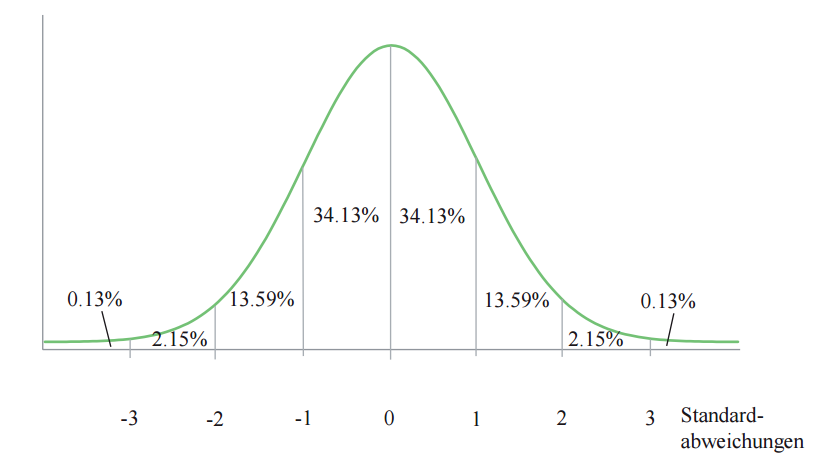
\includegraphics[width = 0.8\textwidth]{Standardabweichung.png}
      \caption{68-95-99,7-Regel\footnote{vgl.: Franz Kronthaler: Statistik angewandt (2014) S. 111 [ge�ndert]}}
  \end{figure}
\end{frame}

\begin{frame}
\frametitle{Dichtefunktion und Standardabweichung}
  \begin{figure}
    \centering
      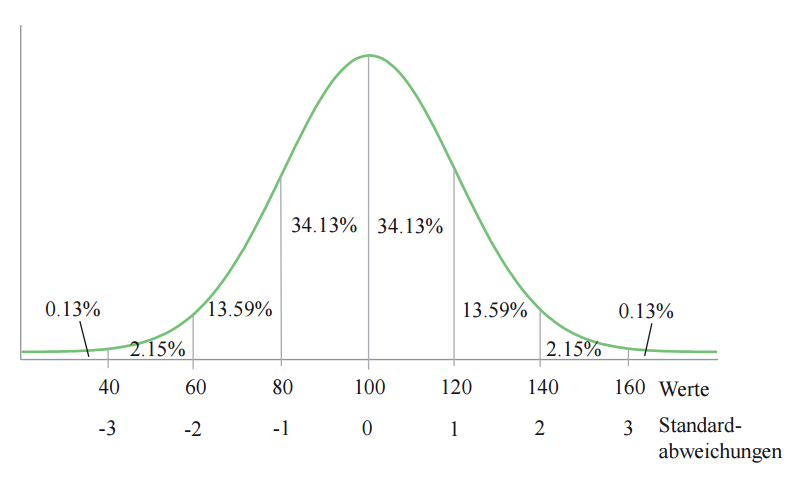
\includegraphics[width = 0.8\textwidth]{Standardabweichung2.png}
      \caption{Fl�chen der Normalverteilung\footnote{Franz Kronthaler: Statistik angewandt (2014) S. 111}}
  \end{figure}
\end{frame}

\begin{frame}
\frametitle{Standardnormalverteilung}
  \begin{figure}
    \centering
      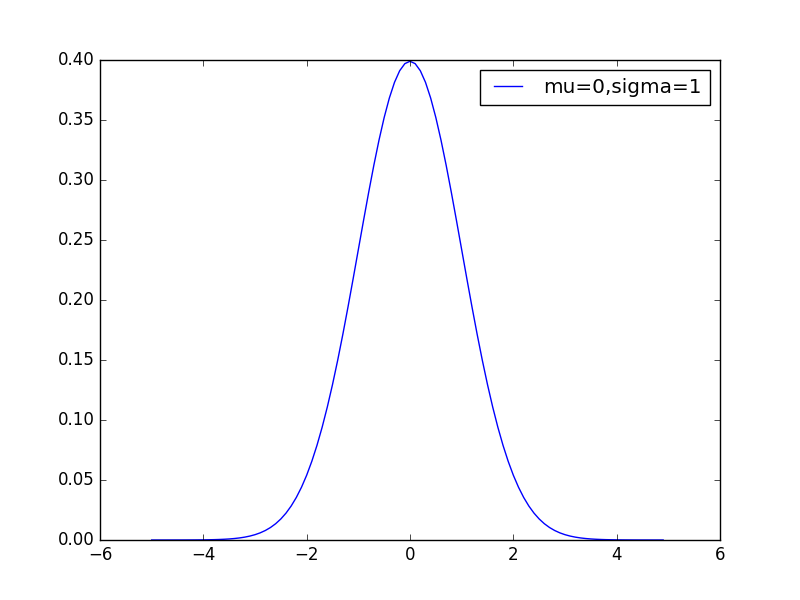
\includegraphics[width = 0.9\textwidth]{Standard.png}
  \end{figure}
\end{frame}

\begin{frame}
\frametitle{Verschiedene Dichtefunktionen normalverteilter Zufallsvariablen}
  \begin{figure}
    \centering
      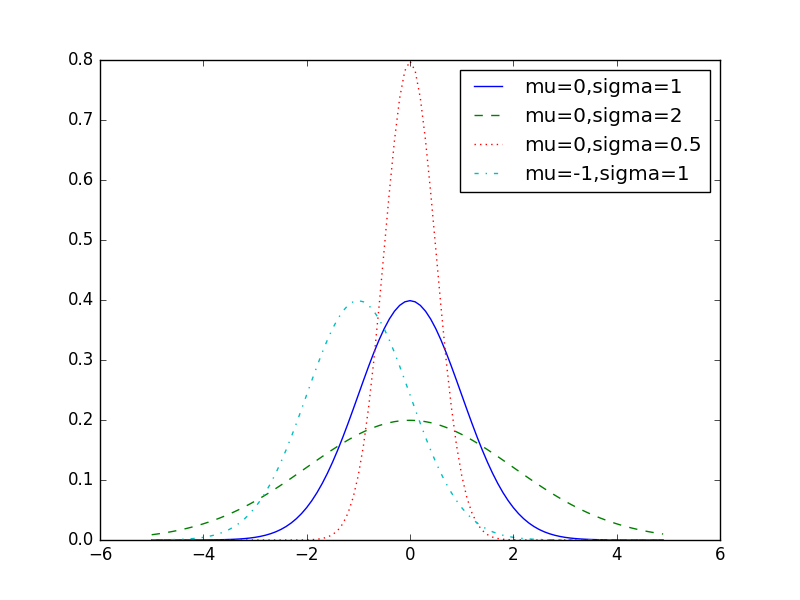
\includegraphics[width = 0.9\textwidth]{Diverse.png}
  \end{figure}
\end{frame}

\begin{frame}
\frametitle{Z-Transformation}
  \begin{block}{}
  F�r jede normalverteilte Zufallsvariable \(X\) gilt: \(Z:=\frac{X-\mu}{\sigma}\),\\
  wobei \(X\) dann in die standardnormalverteilte Zufallsvariable \(Z\) transformiert wurde.
  \end{block}
    \begin{figure}
    \centering
      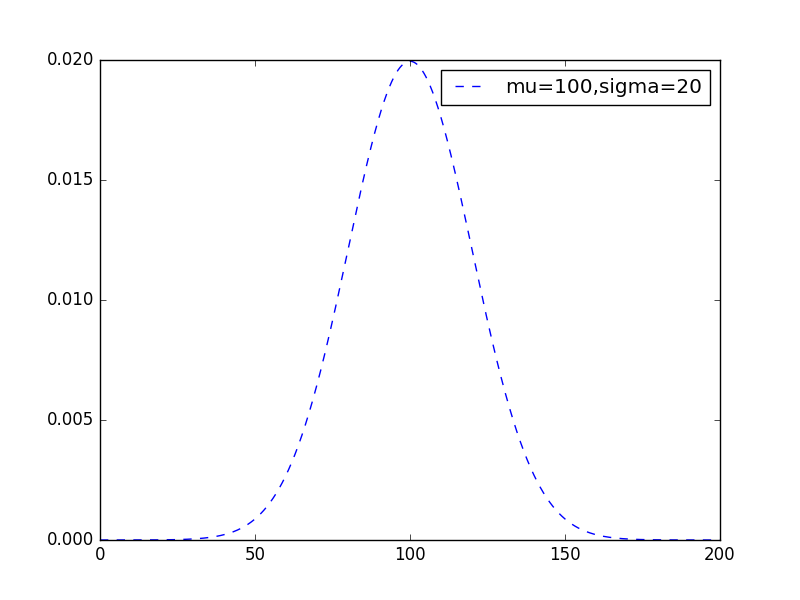
\includegraphics[width = 0.7\textwidth]{ZTransformation.png}
  \end{figure}
\end{frame}

\begin{frame}
\frametitle{Standardnormalverteilung-Tabelle}
  \begin{block}{}
    \begin{equation}
      \Phi_{0,1}(z) = \frac{1}{\sqrt{2\pi}}\int_{-\infty}^{z}e^{-\frac{1}{2}t^2} dt
    \end{equation}
  \end{block}
    \begin{figure}
    \centering
      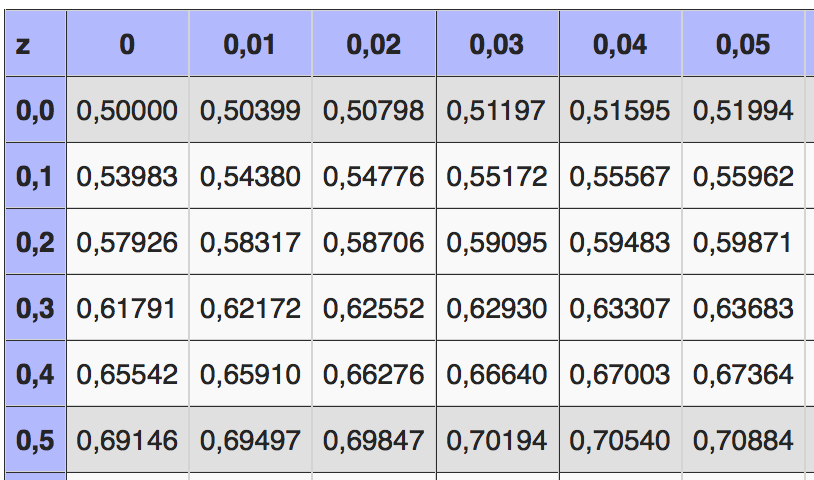
\includegraphics[width = 0.7\textwidth]{Tabelle.png}
      \caption{Wahrscheinlichkeiten\footnote{vgl.: \url{https://de.wikipedia.org/wiki/Tabelle_Standardnormalverteilung}}}
  \end{figure}
\end{frame}

%%%%%%%%%%%%%%%%%%%%%%%%%%%%%%%%%%%%%%%%%%%%
\section{Verteilungsfunktion}

\begin{frame}
\frametitle{Verschiedene Verteilungsfunktionen normalverteilter Zufallsvariablen}
  \begin{block}{}
    \begin{itemize}
      \item \(f(x)\) gibt an, wie hoch die Wahrscheinlichkeit ist, dass der Wert einer Zufallsvariablen \(X\) kleiner oder gleich \(x\) ausf�llt.
      \item existiert f�r jedes positive \(\mu\) und jedes positive \(\sigma\)
    \end{itemize}
  \end{block}
  \begin{figure}
    \centering
      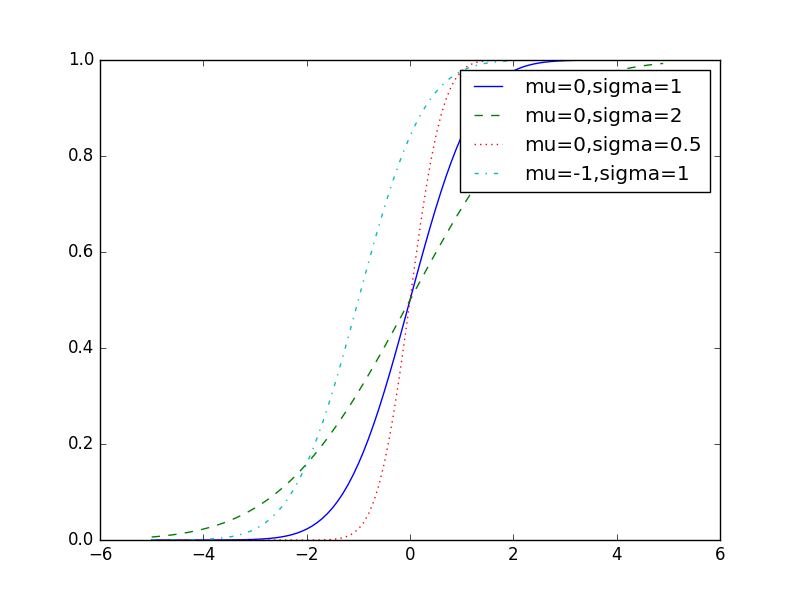
\includegraphics[width = 0.65\textwidth]{Verteilungsfunktion.png}
  \end{figure}
\end{frame}

%%%%%%%%%%%%%%%%%%%%%%%%%%%%%%%%%%%%%%%%%%%%
\section{Anwendung in der Datanalyse}

\begin{frame}
  \frametitle{Anwendung in der Datanalyse}
\end{frame}

\begin{frame}
  \frametitle{Anwendung in der Datanalyse}
  \begin{block}{}
    \begin{itemize}
      \item Anzahl der Bilder, die in einem Jahr erstellt wurden
      \item Anzahl der Bilder pro K�nstler
      \item Anzahl der Bilder pro Land
      \item Anzahl der Tags pro Bild
      \item Anzahl der Taggungen pro Bild
    \end{itemize}
  \end{block}
  \begin{block}{}
    \begin{itemize}
      \item F�llmenge von Lebensmitteln
      \item K�rpergr��e/Schuhgr��e von Menschen
      \item IQ von Menschen
      \item Trinkgeld eines Bar-Mitarbeiters pro Tag
      \item Jahresniederschlag in M�nchen
    \end{itemize}
  \end{block}
\end{frame}

%%%%%%%%%%%%%%%%%%%%%%%%%%%%%%%%%%%%%%%%%%%%
\section{Zentraler Grenzwertsatz}

%\begin{frame}
  %\frametitle{Zentraler Grenzwertsatz}
  %\begin{block}{}
  %Wenn eine Zufallsvariable durch den Mittelwert einer gro�en Menge \(n\) voneinander unabh�ngiger Zufallsvariablen \(x_{1}...x_{n}\) bestimmt wird, die jeweils \textit{gleichm��ig}-normalverteilt sind, so ist auch die zusammengesetzte Zufallsvariable \(X\) nahezu normalverteilt.
    %\begin{equation}
     % X = \frac{1}{n}(x_{1} + ... + x_{n})
    %\end{equation}
  %\end{block}
  %\begin{block}{}
    %\begin{equation}
      %\frac{(x_{1} + ... + x_{n})-\mu*n}{\sigma\sqrt{n}}
    %\end{equation}
  %\end{block}
%\end{frame}

\begin{frame}
\frametitle{Zentraler Grenzwertsatz}
  \begin{block}{}
    \begin{equation}
      X = \frac{1}{n}(x_{1} + ... + x_{n})
    \end{equation}
    Voraussetzungen: 
    \begin{itemize}
      \item \(n\) ist gro�.
      \item \(\mu\) und \(\sigma\) sind f�r \(x_{1} ... x_{n}\) ca. gleich gro�
    \end{itemize}
    Folge: \(\mu(X) \approx \mu(x_{1} ... x_{n})\) und \(\sigma(X) \approx \sigma(x_{1} ... x_{n})\)
  \end{block}
  \begin{figure}
    \centering
      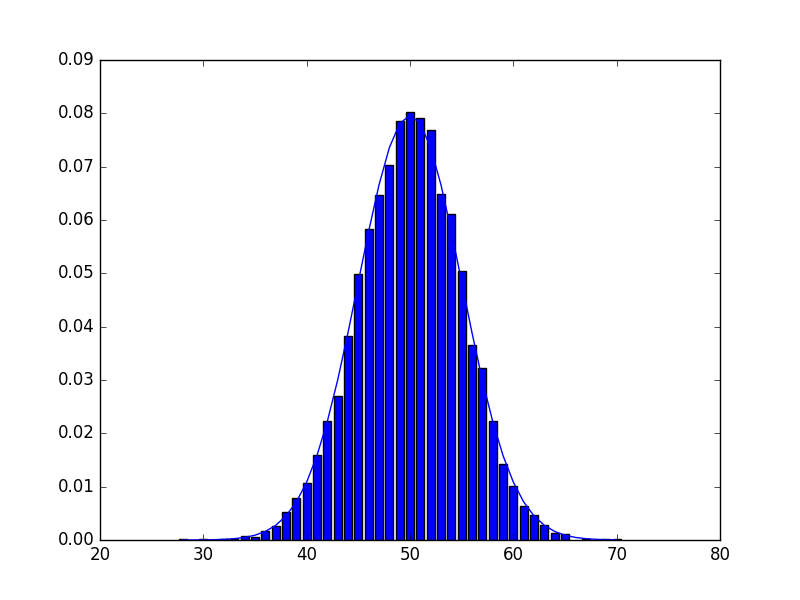
\includegraphics[width = 0.5\textwidth]{vs.png}
  \end{figure}
\end{frame}

%%%%%%%%%%%%%%%%%%%%%%%%%%%%%%%%%%%%%%%%%%%%
\section{Zusammenfassung}

\begin{frame}
  \frametitle{Zusammenfassung}
  \begin{block}{}
    \begin{itemize}
      \item Beschreibung von Zufallsvariablen
      \item Dichte- und Verteilungsfunktion
      \item Standardnormalverteilung: \(\mu = 0\) und \(\sigma = 1\).
      \item Z-Transformation
      \item Grundlage f�r zentralen Grenzwertsatz
    \end{itemize}
  \end{block}
\end{frame}

%%%%%%%%%%%%%%%%%%%%%%%%%%%%%%%%%%%%%%%%%%%%
\section{Quellen}
\begin{frame}
  \frametitle{Quellen}
  \begin{block}{}
    \begin{itemize}
      \item Franz Kronthaler: Statistik angewandt (2014)
      \item Joel Grus: Data Science from Scratch (2015)
      \item Hans-Otto Georgii: Stochastik. Einf�hrung in die Wahrscheinlichkeitstheorie und Statistik (2009)
      \item matheguru.com/stochastik/31-normalverteilung.html
    \end{itemize}
  \end{block}
\end{frame}



\end{document}